\section{Motivation}

    In this section we first motivate online iterative compilation by showing the deleterious effects of choosing the wrong inputs for the
    offline case. Then we go on to show the unsuitability of previously proposed program version comparison metrics.

    \begin{figure}[t!]
        \centering
        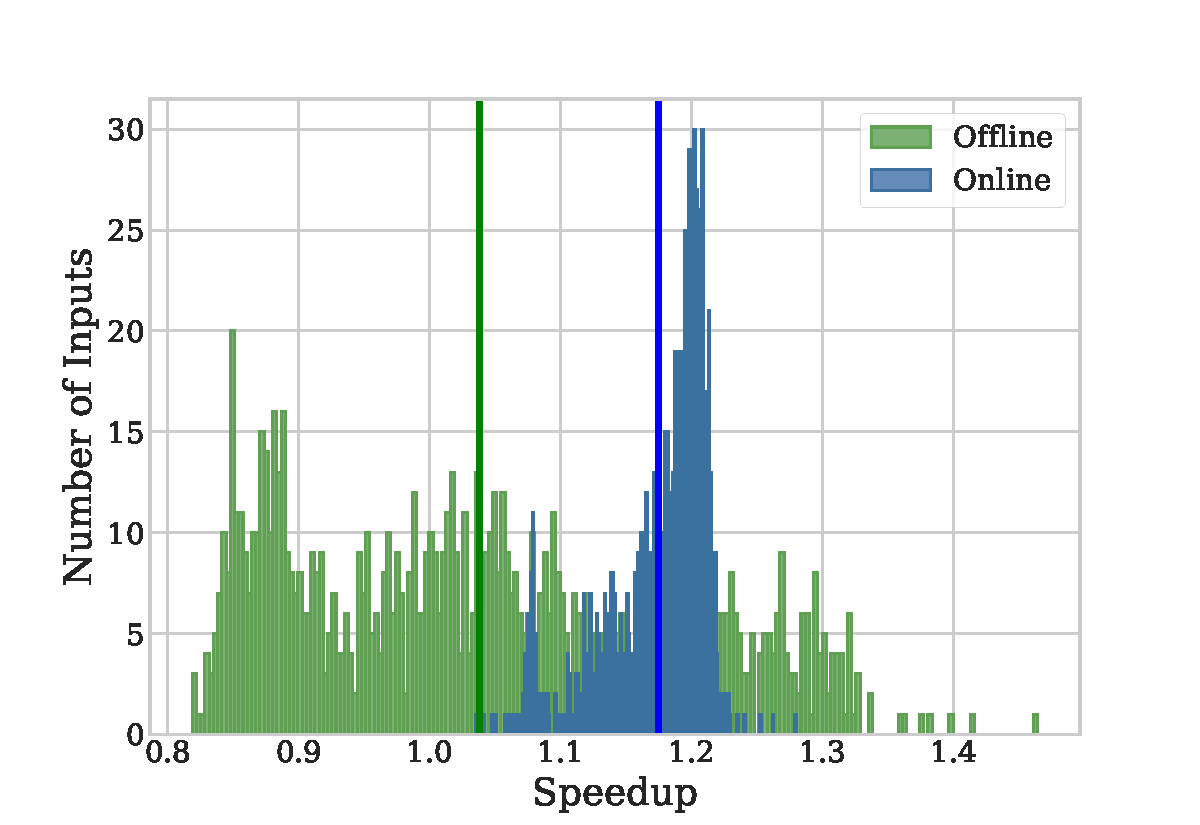
\includegraphics[width=0.5\textwidth]{figs/motivation-online.pdf}
        \caption{
            Histograms of speedup over \texttt{-O3} for each of the 1,000 inputs of \texttt{susan\_c}. The green histogram shows the
            speedup when using the optimization sequence selected by offline \itercomp, the blue one is the speedup using the optimization
            sequence selected by an online-like approach. \FIXME{Beware Daltonism!}
        }
        \label{fig:motivation-online}
    \end{figure}

    We performed offline iterative compilation on \texttt{susan\_c} to find the optimization settings that maximize the average performance
    over \FIXME{five} randomly chosen inputs from a set of 1,000 provided by the \textit{KDataSets} benchmark suite~\cite{chen10,chen12a}.
    The green histogram in Figure~\ref{fig:motivation-online} shows for each of the 1,0000 inputs the speedup versus \texttt{-O3} of that
    chosen optimization setting. The dark green line shows the average speedup for all those inputs. The \FIXME{five} training inputs are
    all in the top \FIXME{twelve} performing inputs. On the other hand, the chosen optimization does poorly on other inputs, often causing
    a slowdown and yielding only a slight speedup of 6\% on average.
    
    The blue bars in Figure~\ref{fig:motivation-online} show a different approach. Here the iterative compilation proceeds by evaluating
    each optimization on \FIXME{five} inputs. Each input is evaluated only once during the search, but the search is provided with oracle
    knowledge about the unoptimized runtime for the inputs, giving a perfect speedup metric. The environment of the search constantly
    changes in the same way as for online iterative compilation. The best optimization for this case never degrades performance compared to
    \texttt{-O3} and is on average 13\% better than the offline approach. The online case, considering truly representative inputs, leads
    to superior performance, if the speedup caused by optimizing can be estimated.

    \begin{figure}[t]
        \centering
        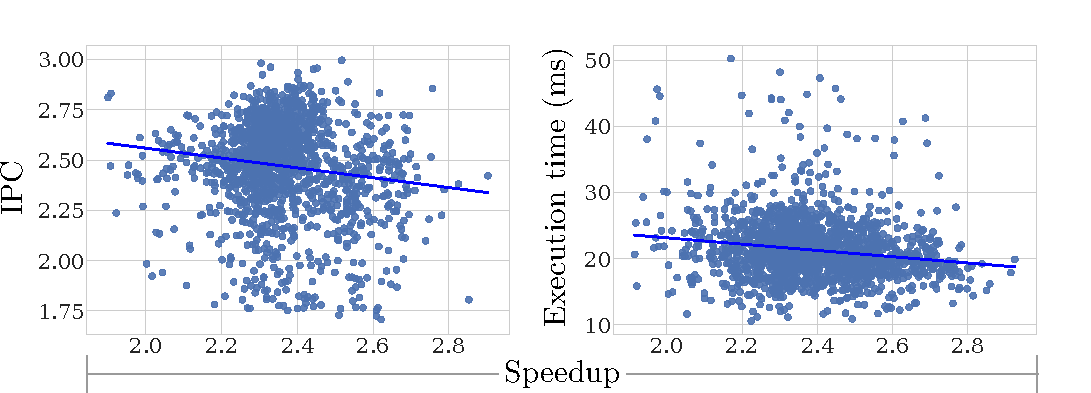
\includegraphics[width=0.5\textwidth]{figs/motivation-metric.pdf}
        \caption{
            Relationship between IPC and execution time vs optimization speedup for 500 different binaries of \texttt{susan\_c}.
            Each point represents averages over a subset of all inputs.
        }
        \label{fig:motivation-metric}
    \end{figure}
    
    Prior to this paper there were two proposed metrics to correlate with program efficiency. The first is simply to use runtime, ignoring
    the work aspect. This functions well when the inputs all require similar effort. When that is not the case it bears little or no
    correlation to efficiency. The second approach is \textit{instructions per cycle}~(IPC), suggested by~\citep{fursin07}. While IPC seems
    promising in the sense that faster instruction execution is a good thing, this is belied by the simple observation that adding
    redundant NOPs to a program will increase IPC while also slowing the program down. Figure~\ref{fig:motivation-metric} shows the
    relationship between execution time, IPC and speedup for different optimizations of \texttt{susan\_c}, averaged across a subset of the
    inputs. Neither IPC nor execution time correlate well, and so neither can be used for iterative compilation. We need a work efficiency
    metric which can approximate speedup instead, using only a single execution.

    In the remainder of this paper we present our work efficiency metric and demonstrate its utility for iterative compilation.
